% The dvipsnames option is passed to the xcolor package, which beamer loads
\documentclass[xcolor={dvipsnames}]{beamer}

\usepackage{smpa2152-style}

\title[OLS Regression]{Ordinary Least Squares (OLS) Regression}
\author[DATA 3100]{DATA 3100}
\date{Prof. Bell}

\begin{document}

%%%%%%%%%%%%%%%%%%%%%%%%%%%%%%%%%%%%%%%%%%%%%%%%%%%%%%%%%%%%%%%%%%
\frame{
\titlepage
}

%%%%%%%%%%%%%%%%%%%%%%%%%%%%%%%%%%%%%%%%%%%%%%%%%%%%%%%%%%%%%%%%%%
\frame{\frametitle{What is Regression?}

\only<1-5,9>{
    \begin{itemize}[<+->]
        \item So far, we've learned how to compare the mean of two groups using a \textbf{t-test}
        \item But often, a t-test is too restrictive for the analysis we want to conduct:
        \begin{itemize}
            \item What if we have two continuous variables? Income, age, and years of education are common variables that we may not want to force into two discrete categories.
            \item What about \textbf{confounders}? ~\\
            \begin{block}{Confounder}
            A variable that explains change in both the independent and dependent variable.
            \end{block}
            \item When we fail to account for confounders, we face \textbf{omitted variable bias} and our estimates are not accurate.
        \end{itemize}
    \end{itemize}
}
\only<6>{
    \centering
    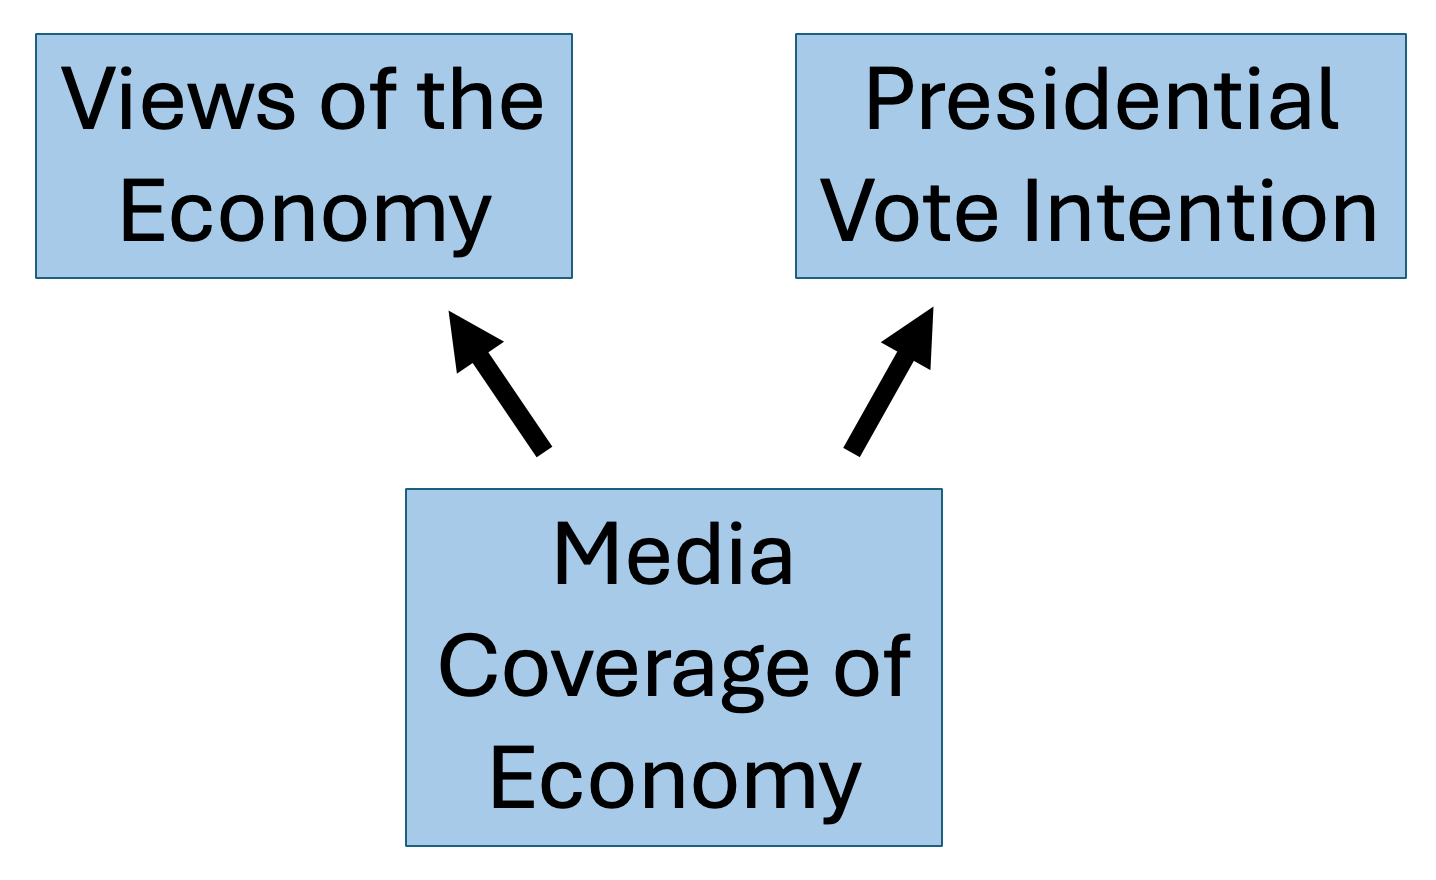
\includegraphics[width=.9\textwidth]{confounding.png}
}
\only<7>{
    \centering
    \textbf{"It's most dangerous to launch fireworks in July."} \\
    IV: Time \\
    DV: Fireworks-related hospitalizations \\
    ~\\
    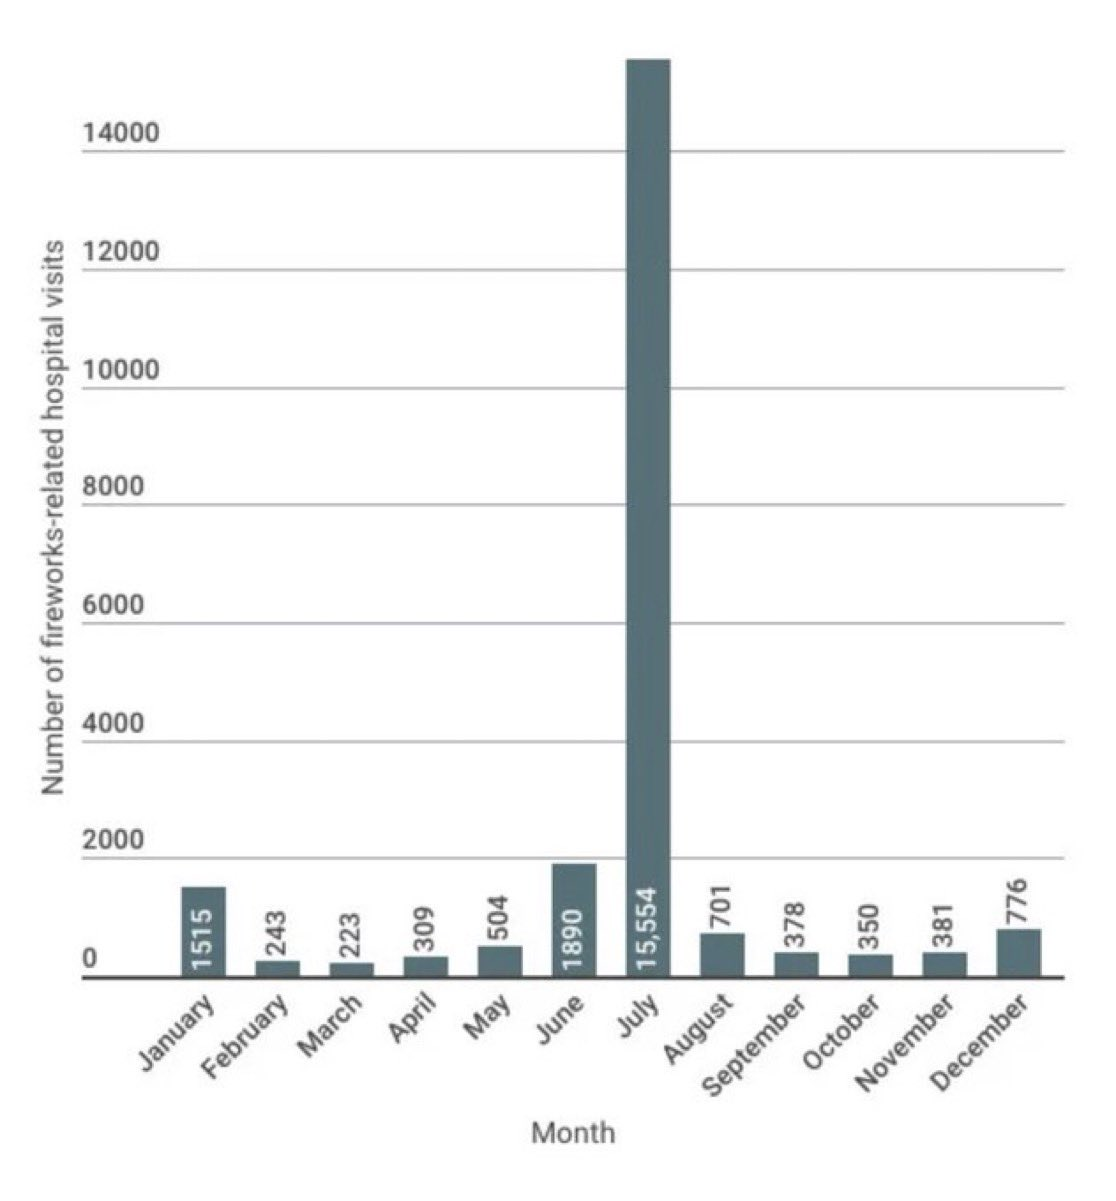
\includegraphics[height=.6\textheight]{firework_injuries.jpeg}
}
\only<8>{
    \centering
    \textbf{"If aliens exist, they will arrive on July 4th."} \\
    IV: Time \\
    DV: UFO Sightings \\
    ~\\
    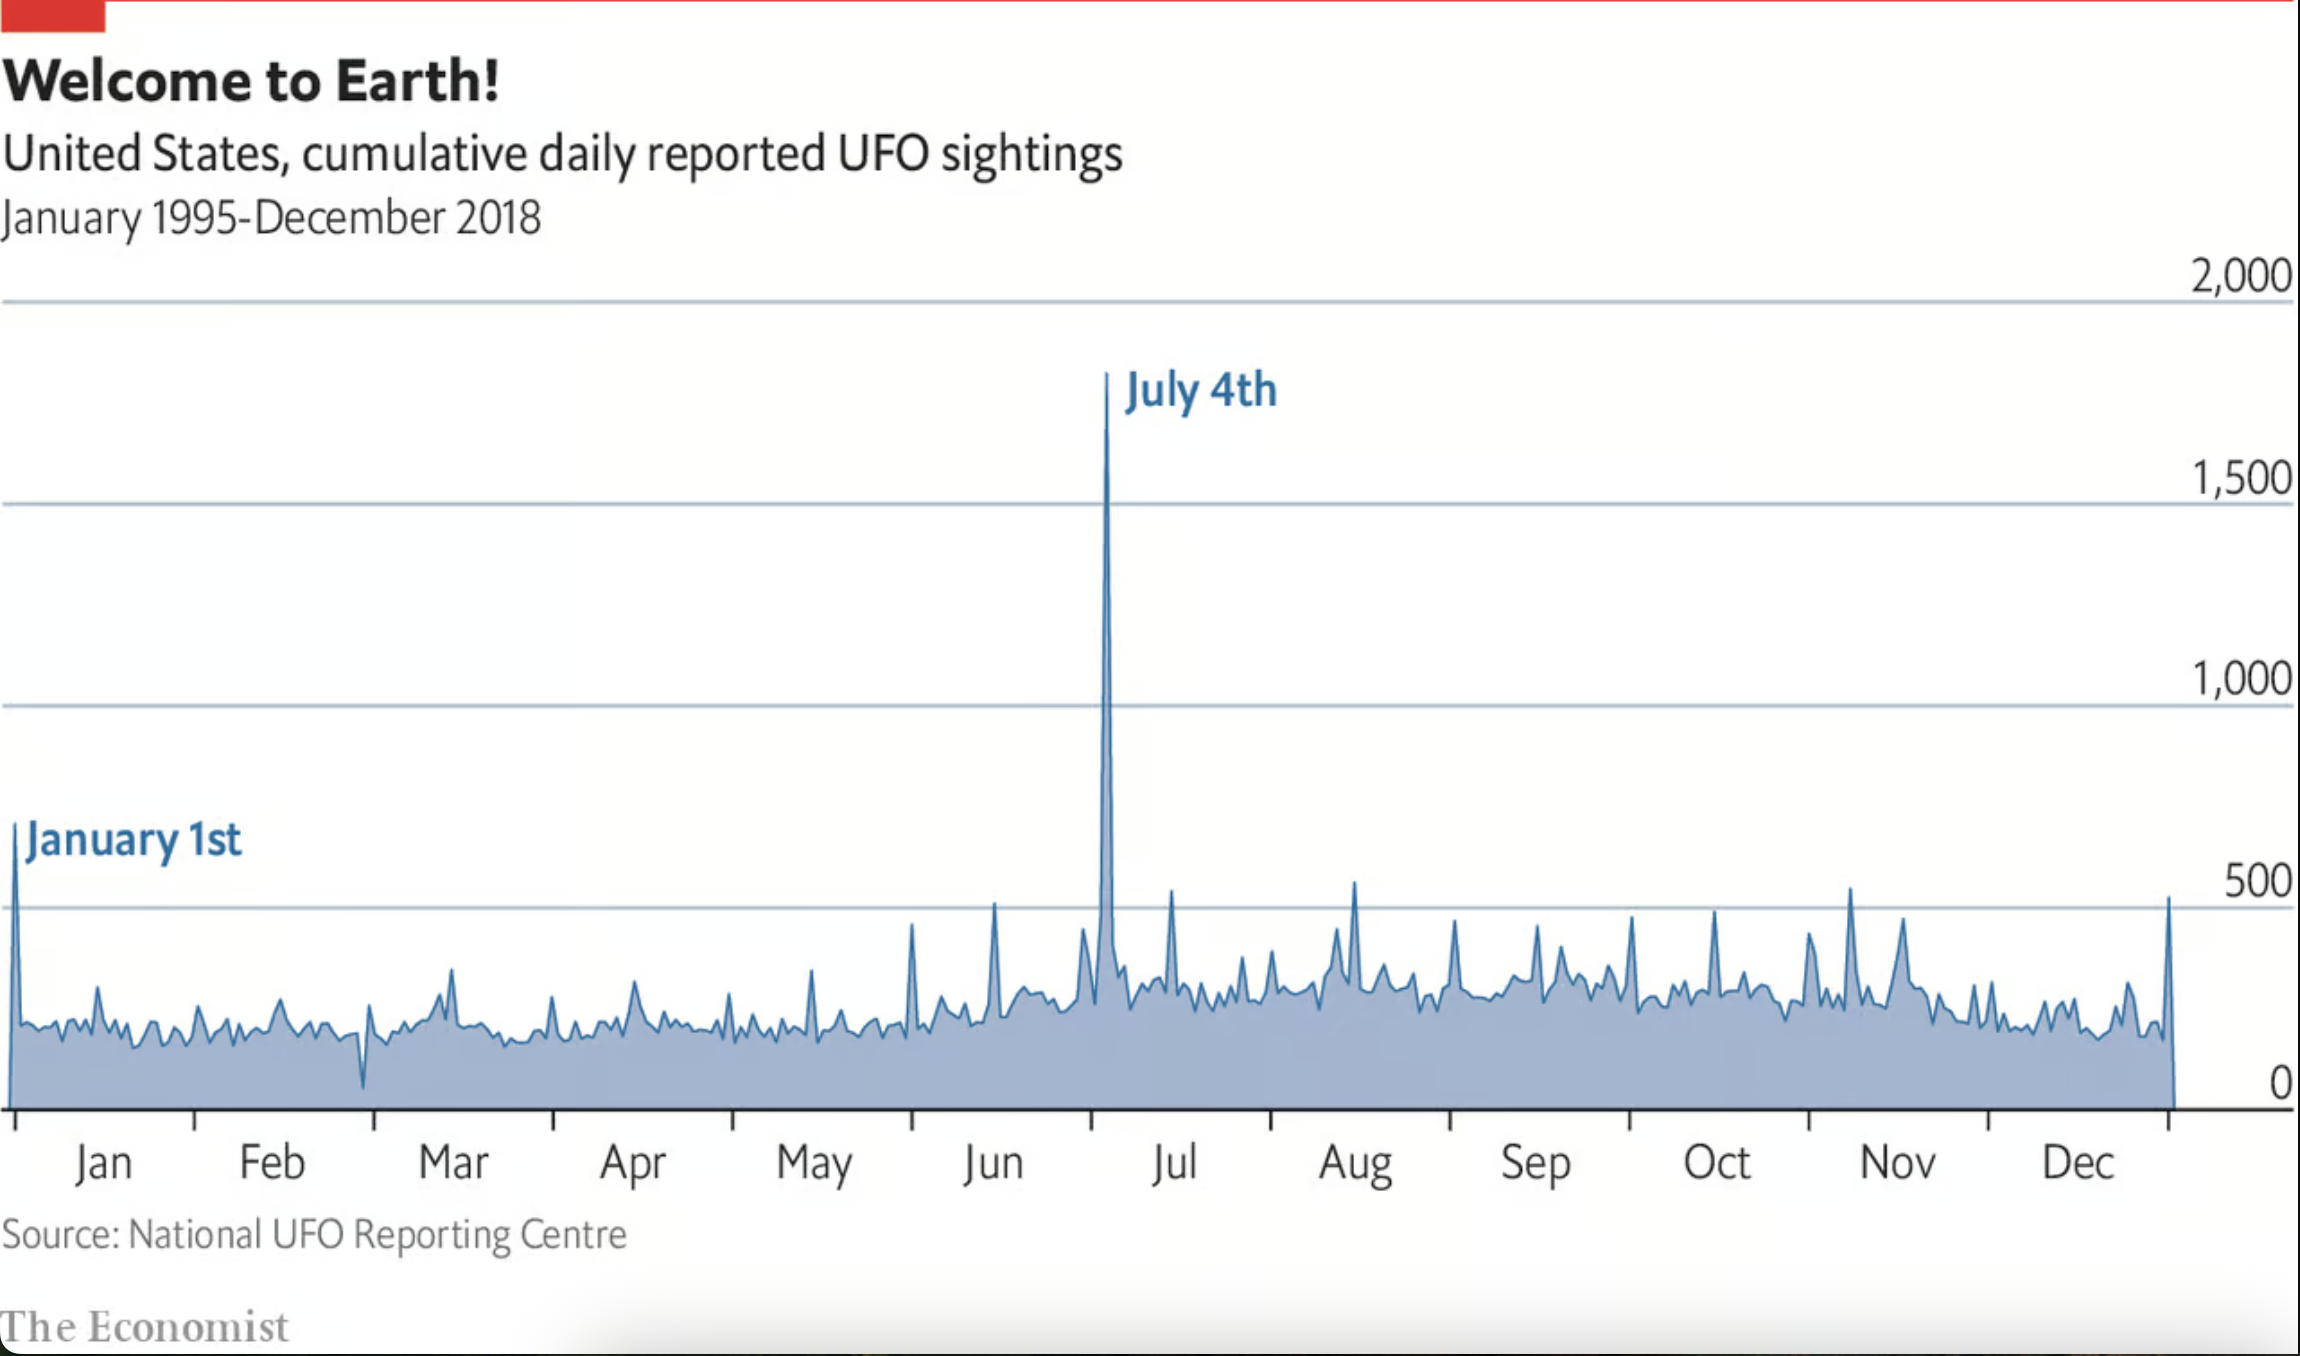
\includegraphics[width=.7\textwidth]{ufo_sightings.png}
}
}

%%%%%%%%%%%%%%%%%%%%%%%%%%%%%%%%%%%%%%%%%%%%%%%%%%%%%%%%%%%%%%%%%%
\frame{\frametitle{Estimating the Regression (Best Fit) Line}
\only<1-3>{The linear regression equation is:
\begin{center}
$Y = \beta_0 + \beta_1X + \epsilon$\\
~\\
$Y$ = dependent variable\\
$\beta_0$ = intercept\\
$\beta_1$ = slope, also called a coefficient\\
$X$ = independent variable\\
$\epsilon$ = error
\end{center}}

\only<2-3>{This looks very similar to a linear equation you might have learned before:
\begin{center}
$y = ax + b$\\
\only<3>{$y = b + ax$}
\end{center}}
}

%%%%%%%%%%%%%%%%%%%%%%%%%%%%%%%%%%%%%%%%%%%%%%%%%%%%%%%%%%%%%%%%%%
\frame{\frametitle{Example}

You want to estimate the effect of income on the allocation to welfare applicants. The linear regression equation is:
\begin{center}
$\hat{Allocation} = \hat{\beta}_0 + \hat{\beta}_1Income$
\end{center}

The \enspace  $\hat{}$ \enspace is the mathematical notation for ``estimate of the mean''\\
~\\
\only<2->{If ``Income'' in thousands has a value of 100, and the intercept is \$605, and the coefficient is -.5, what is our estimated mean of ``Allocation''?}

\only<3->{\begin{center}
$\hat{Allocation} = 605 + (-.5)*100$
\end{center}}

\only<4->{\begin{center}
$\hat{Allocation} = 555$
\end{center}}

\only<5>{So the coefficient ($\beta_1$) is the effect of a \textbf{one-unit} change in income (thousands) on the mean allocation.}
}

%%%%%%%%%%%%%%%%%%%%%%%%%%%%%%%%%%%%%%%%%%%%%%%%%%%%%%%%%%%%%%%%%%
\frame{\frametitle{What Is Error?}
\only<1>{Recall that the linear regression equation is:
\begin{center}
$Y = \beta_0 + \beta_1X + \epsilon$\\
~\\
$Y$ = dependent variable\\
$\beta_0$ = intercept\\
$\beta_1$ = slope, also called a coefficient\\
$X$ = independent variable\\
$\epsilon$ = error
\end{center}}
\only<3>{\centering
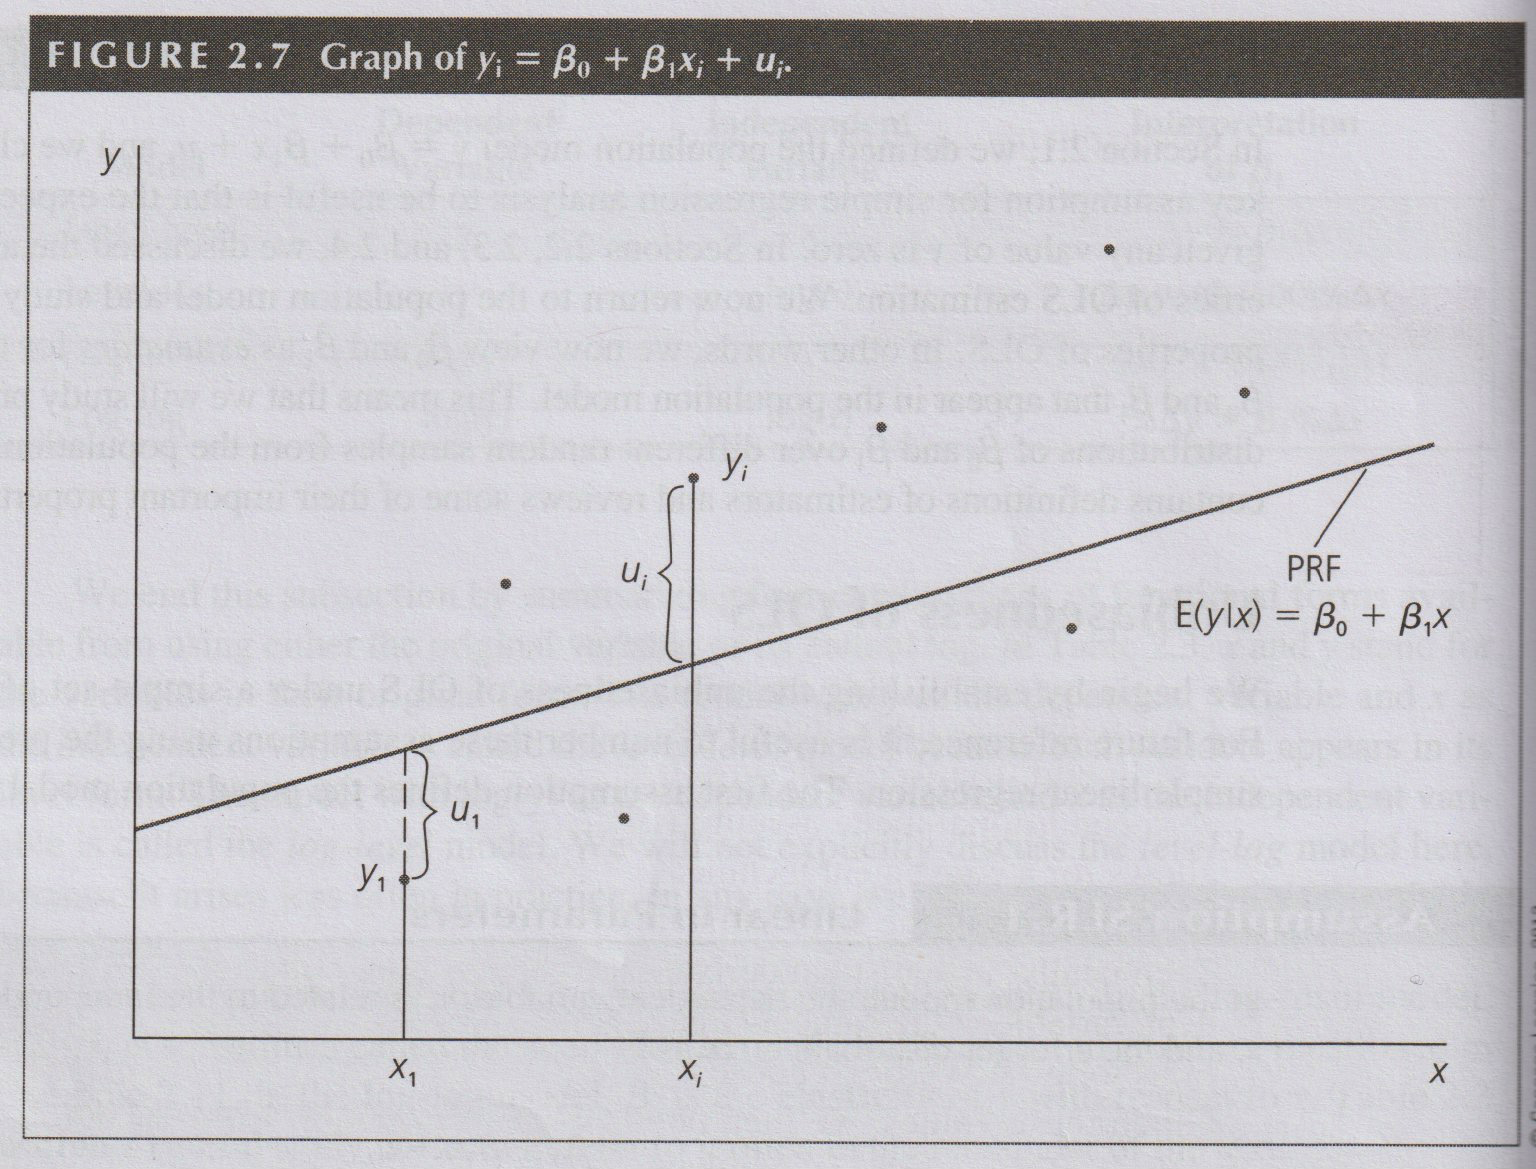
\includegraphics[width=.8\textwidth]{RegressionError.png}}
\only<2,4->{\begin{itemize}[<+->]
    \item Error ($\epsilon$ or $u$) is also called the residual (left over from $Y = \beta_0 + \beta_1X$, our best fit line)
    \item<3-> Our goal in regression is to fit the best line that  minimizes the error
    \item<5> However, we can never get the $\epsilon$ = 0, and often we don't even get close. We just do the best we can to make the ``best'' best fit line.
\end{itemize}}
}

%%%%%%%%%%%%%%%%%%%%%%%%%%%%%%%%%%%%%%%%%%%%%%%%%%%%%%%%%%%%%%%%%%
\frame{\frametitle{Multiple Linear Regression}
\only<1-3>{The multiple linear regression equation is:
\begin{center}
$Y = \beta_0 + \beta_1X_1 + \beta_2X_2 + \epsilon$\\
~\\
$Y$ = dependent variable\\
$\beta_0$ = intercept\\
$\beta_i$ = slope coefficient\\
$X_i$ = independent variable\\
$\epsilon$ = error
\end{center}
\only<2>{\textcolor{blue}{What is the interpretation of $\beta_1$?}\\
~\\
$\beta_1$ is the effect of a one-unit change in $X_1$ on the mean of $Y$, holding $X_2$ constant (the independent effect of $X_1$ on $Y$)}
\only<3>{\textcolor{blue}{What is the interpretation of $\beta_2$?}\\
~\\
$\beta_2$ is the effect of a one-unit change in $X_2$ on the mean of $Y$, holding $X_1$ constant (the independent effect of $X_2$ on $Y$)}}
}

%%%%%%%%%%%%%%%%%%%%%%%%%%%%%%%%%%%%%%%%%%%%%%%%%%%%%%%%%%%%%%%%%%
\frame{\frametitle{Non-Continuous Dependent Variables}
\begin{itemize}[<+->]
    \item One of the assumptions of linear regression is that the relationship between $X$ and $Y$ is linear (you can draw a best fit line)
    \item This assumption is usually fine when we are working with continuous dependent variables like income
    \item What about categorical dependent variables, like party ID? The linear regression model is not well suited for these.
    \item What about binary dependent variables, like support for a policy?\\
    ~\\
    We call this a linear probability model because it estimates the effect of a one-unit change in $X$ on the \textit{probability} (percent chance) of a value of ``1'' for the dependent variable
\end{itemize}
}

\end{document}
